\documentclass[]{article}
\usepackage[a4paper, total={6.5in, 8.5in}]{geometry}
\usepackage{hyperref}
\usepackage{amsmath}
\usepackage{amssymb}
\usepackage{graphicx}
\usepackage{float}
\usepackage{algorithm}
%\usepackage{algorithmic}
\usepackage{algpseudocode}

\title{Towards Comparable Active Learning}

\begin{document}

\maketitle

\section{Introduction}


\subsection{Contribution}

\section{Related Work}

\section{Overview}


\subsection{Problem Description / Delineation}
\textbf{Basic Classification}\\
We assume a dataset $\mathcal{D} := (x_i, y_i) \hspace{0.5mm}; \hspace{1mm} i := 1 \ldots N$ consisting of instances $x_i \in \mathbb{R}^M$ and corresponding $y_i \in \mathbb{R}^C$.
For evaluation purposes we assume a held-out test set $\mathcal{D}^{\text{test}}$ with the same characteristics.
We consider classification problems with one-hot encoded classes, hence $C$ models the number of classes.
To perform classification, a model $\hat y_\theta : \mathbb{R}^M \rightarrow \mathbb{R}^C$ is used. To fit the model, it is parameterized by $\theta$ and subjected to loss $\ell: \mathbb{R}^C \times \mathbb{R}^C \rightarrow \mathbb{R}$. For this work, categorical cross-entropy (CE) is used.
For evaluating classification performance, we use accuracy on the test set $\operatorname{Acc}(\mathcal{D}^{\text{test}}, \hat{y}_\theta)$. \\ [1mm]
%
\textbf{Pool-based AL with single instances (non-batch setting)}\\
To construct the active learning setting, we suppress the labels $y_i$ of $\mathcal{D}$ to form the unlabeled pool $\mathcal{U} := u_i \hspace{0.5mm}; \hspace{1mm} i := 1 \ldots N$ and form and initial labeled pool $\mathcal{L}$ by uniformly sampling $k$ number of instances per class from $\mathcal{U}$ and recovering their label. 
The result of this so-called "seeding" process is $\mathcal{L} := (u_i, y_i) \hspace{0.5mm}; \hspace{1mm} i := 1 \ldots k*C$. \\
Active learning is defined as sequentially removing single instances $u^{(i)} \in \mathcal{U}^{(i)}\hspace{1mm}; \hspace{2mm} \mathcal{U}^{(i+1)} := \mathcal{U}^{(i)} \setminus´ \{u^{(i)}\}$, recovering their label $y^{(i)}$ and adding them to the labeled pool $\mathcal{L}^{(i+1)} := \mathcal{L}^{(i)} \cup (u^{(i)}, y^{(i)})$ until a fixed budget $B$ is exhausted $i := 1 \ldots B$.
After each added instance the classification model is retrained according to section \ref{sec:training_the_classifier} and its performance is measured on the held-out test set $\mathcal{D}^{\text{test}}$.
The quality of an active learning algorithm is evaluated by an "anytime" protocol that incorporates classification performance at every iteration, not just the final performance after the budget is exhausted.
We employ the normalized area under the accuracy curve (AUC):
\begin{equation}
	\operatorname{auc}(\mathcal{U}, \mathcal{L}, \hat y, B) := \frac{1}{B} \sum_{i=1}^{B} \operatorname{Acc}(y_{test}, \hat y_i(x_{test}))
\end{equation}
Where $\hat y_i$ is the retrained classification model after the i-\textit{th} instance was selected. \\ [1mm]
%
\textbf{Framing AL as RL}\\
We define the active learning process as an adapted reinforcement learning loop $(S, A, \tau, \Omega, \omega)$ where an environment iteratively will expose a state $s \in S$ to an agent $\Omega$, which will choose actions $a \in A$.
For each iteration $i$ the environment samples a subset of size $\tau$ of unlabeled instances $u^{(i)} \underset{\tau}{\sim} \mathcal{U}^{(i)}$, constructs the state $s^{(i)} := \omega(u^{(i)})$ and presents it to the agent to select an action $a^{(i)} := \Omega(s^{(i)})$.
The action $a^{(i)}$ is the index of the selected instance in $u^{(i)}$ out of all possible indices $A := [1 \ldots \tau]$.
This process is repeated $B$ times $i := [1 \ldots B]$.

\begin{minipage}{0.59\linewidth}
	\begin{algorithm}[H]
		\caption{Active Learning}\label{alg:active_learning}
		\begin{algorithmic}[1]
			\Require $\mathcal{U}$ \Comment{Unlabeled Pool}
			\Require $\tau$ \Comment{Unlabeled Sample Size}
			\Require $\Omega$ \Comment{AL Agent}
			\Require $\omega$ \Comment{Environment State function}
			\State $\mathcal{L}^{(1)} \gets \operatorname{seed}(\mathcal{U})$  \Comment{Create the initial labeled set}
			\State $\mathcal{U}^{(1)} \gets \mathcal{U}$
			\For{$i := 1 \ldots B$}
			\State $u^{(i)} \underset{\tau}{\sim} \mathcal{U}^{(i)}$
			\State $s^{(i)} \gets \omega(u^{(i)})$
			\State $a^{(i)} \gets \Omega(s^{(i)})$ \Comment{$a^{(i)}$ is an index inside of $u^{(i)}$}
			\State $y^{(i)} \gets \operatorname{oracle}(u^{(i)}_{a})$ \Comment{$u^{(i)}_{a}$ is shorthand for $u^{(i)}_{a^{(i)}}$}
			\State $\mathcal{L}^{(i+1)} \gets \mathcal{L}^{(i)} \cup \{(u^{(i)}_a, y^{(i)})\}$
			\State $\mathcal{U}^{(i+1)} \gets \mathcal{U}^{(i)} \setminus \{u^{(i)}_a\}$
			\State $\text{acc}^{(i)} \gets \operatorname{Retrain}(\mathcal{L}^{(i+1)})$  \Comment{$\operatorname{Retrain}(\mathcal{L}^{(i+1)})$ is shorthand for $\operatorname{Retrain}(\mathcal{L}^{(i+1)}, \mathcal{L}^\text{test}, \hat y_\theta, e^\text{max})$}
			\EndFor
			\State
			\Return $\frac{1}{B} \sum_{i=1}^{B} \text{acc}^{(i)}$
		\end{algorithmic}
	\end{algorithm}
\end{minipage}
\hspace{3mm}
\begin{minipage}{0.35\linewidth}
	\begin{algorithm}[H]
		\caption{Retrain}\label{alg:retrain}
		\begin{algorithmic}[1]
			\Require $\mathcal{L}$ \Comment{Labeled Pool}
			\Require $\mathcal{L}^\text{test}$ \Comment{Labeled Test Data}
			\Require $\hat y_\theta$ \Comment{Classification Model}
			\Require $e^\text{max}$ \Comment{Maximum Epochs}
			\State $\text{loss}^* \gets \infty$
			\For{$i := 1 \ldots e^{\text{max}}$}
			\State $\theta_{i+1} \gets \theta_i - \eta \nabla_\theta \ell(\mathcal{L}, \hat y_{\theta})$
			\State $\text{loss}_i \gets \ell(\mathcal{L}^\text{test}, \hat y_{\theta})$
			\If{$\text{loss}_i < \text{loss}^*$}
			\State $\text{loss}^* \gets \text{loss}_i$
			\Else
			\State Break
			\EndIf
			\EndFor
			\State
			\Return Acc($\mathcal{L}^\text{test}, \hat y_{\theta}$)
		\end{algorithmic}
	\end{algorithm}
\end{minipage}




\section{Methodology}

\subsection{Classification Model}
The classifier is constructed according to two kinds of information.
The general class of model (Dense, Convolutional, Attention, ...), and the configuration of the model (number of layers, size of each layer, ...). \\
The model class and exact configuration is determined by the dataset, i.e. tabular datasets will prescribe a dense model.
If special capabilities of the model are needed (i.e. Monte-Carlo Dropout), an extension of the given model class can be provided to the framework. \\ [1mm]
To ensure comparability between models, the model's configuration should not be changed or an additional evaluation of the new configuration should be conducted to compare the baseline expressivity.

\subsection{State Space}
Since every AL agent needs a different state space our environment exposes a callback-function that gives the agent full control over how the state is constructed. \\ [1mm]
The callback includes the following information:
\begin{itemize}
	\item The current sample of IDs that point to the presented unlabeled datapoints
	\item The entire labeled dataset $\mathcal{L}$
	\item The entire unlabeled dataset $\mathcal{U}$
	\item A histogram of labeled points per class (count)
	\item The available budget
	\item Number of added datapoints $|\mathcal{L}| - |\mathcal{S}|$
	\item The initial validation accuracy and current validation accuracy
	\item The current classification model including all model weights
	\item The current optimizer including it's full state
\end{itemize}
Every agent needs to implement this callback that transforms the given information into a state tensor that will be directly consumed by the agent to make it's prediction.

\subsection{Training the Classifier}\label{sec:training_the_classifier}
\subsection{Evaluation}\label{sec:evaluation}


\section{Ablation Studies}
\begin{itemize}
	\item Weird drop of performance for multiples of batch size (drop\_last in DataLoader)
	\item Reduction of the test set for speed
\end{itemize}


\bibliographystyle{plain}
\bibliography{main.bib} 

\appendix

\section{Comparison of different sample sizes $\tau$}
\begin{figure}[H]
	\centering
	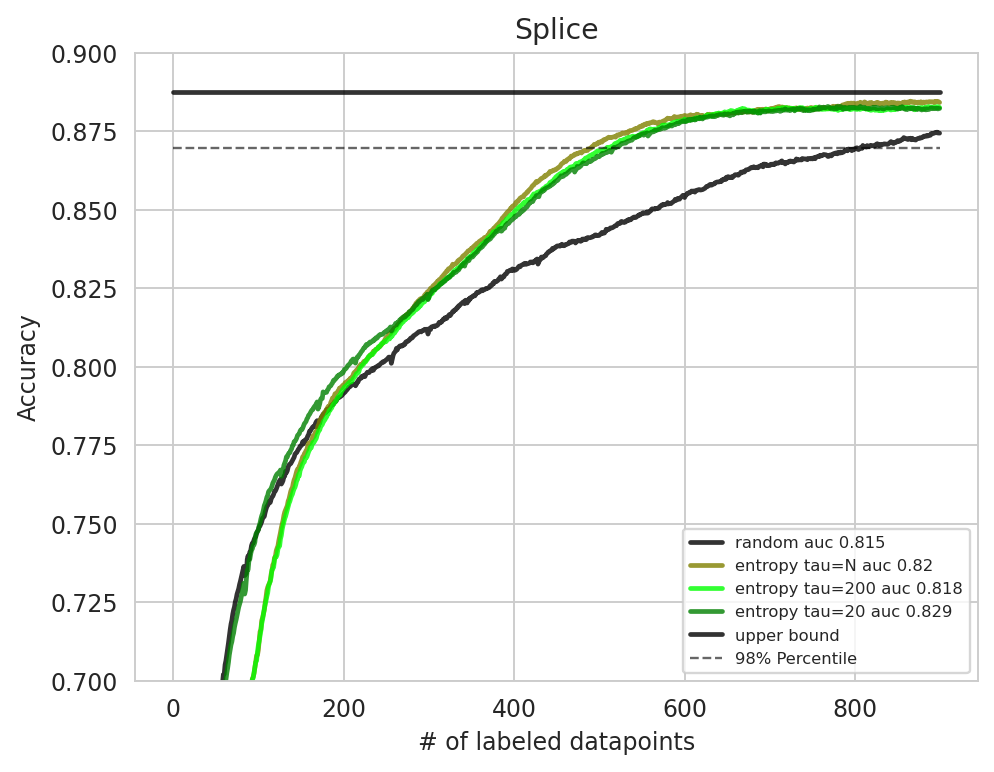
\includegraphics[width=0.7\linewidth]{img/tau_ablation.png}
\end{figure}

\end{document}